\documentclass[a4paper,11pt,uplatex]{jsbook}

%\usepackage{fancyhdr}
\setlength{\footskip}{16pt}
\usepackage{amsmath}
\usepackage[dvipdfmx]{graphicx}
\usepackage[dvipdfmx]{color}
%\usepackage{pagecolor}[white]
\usepackage{amsmath,amssymb}
%\usepackage[top=3cm, bottom=3cm, left=3cm, right=3cm]{geometry}
\usepackage{braket}
\usepackage{bm}
\numberwithin{equation}{section}
\usepackage{mathrsfs}
\usepackage{siunitx}
\usepackage{physics}
\usepackage[dvipdfmx]{graphicx}
\usepackage[compat=1.1.0]{tikz-feynhand}
\usepackage{caption}
\usepackage{subcaption}
%\usepackage{cleveref}
\usepackage{float}
\usepackage{multicol}
\setlength{\columnsep}{15mm}
%\usepackage[style=phys,articletitle=false,biblabel=brackets,chaptertitle=false,pageranges=false]{biblatex}
%\usepackage[style=phys]{biblatex}
\usepackage[dvipdfmx]{hyperref}
\usepackage{url}
\usepackage{pxjahyper}
\usepackage{bookmark}
%\usepackage[backref]{hyperref}
\setcounter{tocdepth}{3}
\setlength{\parindent}{2em}
\def\vector#1{\mbox{\boldmath $#1$}}
\def\slash#1{\not\!#1}
\def\slashb#1{\not\!\!#1}
\def\delsla{\not\!\partial}
%\usepackage[dvipdfmx]{xcolor}


\hypersetup{
 setpagesize=false,
 bookmarksnumbered=true,%
 bookmarksopen=true,%
 colorlinks=true,%
 linkcolor=black,
 citecolor=red,
 urlcolor=black,
}
%backreferenceのカスタマイズ. "Back to p.3"のように表示する.
%\renewcommand*{\backref}[1]{(p.#1へ戻る)}
%\newcommand{\backtoc}{\hyperlink{toc}{[目次へ]}}
\newcommand{\backtoc}{\texorpdfstring{\protect\hyperlink{toc}{\hspace{5pt} \scriptsize [目次へ]}}{}}
\newcommand{\mychapter}[1]{\chapter[#1]{#1\backtoc}}
\newcommand{\mysection}[1]{\section[#1]{#1\backtoc}}
\newcommand{\mysubsection}[1]{\subsection[#1]{#1\backtoc}}
% 数式
%\usepackage{amsmath,amsfonts}
%\usepackage{bm}
%\usepackage{physics}
%\usepackage{siunitx}
% 画像
%\usepackage[dvipdfmx]{graphicx}
%\usepackage[dvipdfmx,colorlinks=true,linkcolor=blue]{hyperref}
%\usepackage{pxjahyper}

\begin{document}

\chapter{導入}
\section{ハイパー核}
本論文は、ドイツ、マインツ大学にある連続電子線加速器マインツマイクロトロン(MAMI)における200 MeV領域の電子ビームエネルギー測定について論じる。
電子ビームエネルギーの絶対値を$\delta \text{E}/\text{E} \sim 10^{-4}$の精度で測定し、磁気運動量スペクトロメータの系統誤差を$\delta p/p \sim 10^{-4}$に抑えることで、
過去に我々が測定した$^4_{\Lambda} \text{H}$における$\Lambda$粒子の束縛エネルギーの精度$100$ keVから向上させ、
ハイパートライトン$^3_{\Lambda}\text{H}$における$\Lambda$束縛エネルギーを10 keVを切る精度で決定することを目指す。
ハイパートライトンにおける$\Lambda$束縛エネルギーの決定精度向上は、$\Lambda$N相互作用に対しさらなる知見を与える。\\
本章でははじめにハイパー核とその研究の歴史、ハイパー核生成実験について述べる。次に我々がマインツマイクロトロンにおいて独自に開発した$\Lambda$ハイパー核精密質量分光手法である
崩壊パイ中間子法とその課題となっている電子ビームエネルギー測定精度の重要性について述べた後、最後に本研究の目的を述べる。

\subsection{ハイペロンとハイパー核}
素粒子の標準理論によれば、自然界の粒子は全てそれ以上分割できない最小単位の粒子(素粒子)からなり、素粒子の間に働く力は、強い力、弱い力、電磁気力、重力の4種類の力であると理解されている。
素粒子は物質を構成する粒子と力を媒介する粒子に分類でき、さらに物質を構成する粒子は強い相互作用をするクォークと強い相互作用をしないレプトンに分類できる。
クォークは表に示すように三世代に分類されている。\\
クォークは単体で存在することはできず、3つ集まったハドロンが2つ集まったメソンの形で存在する。我々の身の回りの物質はハドロンである陽子と中性子からなる原子核と、その周りを囲む電子からなる原子によって構成されている。
陽子、中性子は特に通常原子核を構成する意味で核子(Neucleon)と呼ばれている。
陽子はuudクォーク、中性子はuddクォークからなり、それぞれ電荷+1と0を持つ。クォークにはそれぞれアイソスピンと呼ばれる量子数を導入することでスピン演算子と同じ枠組みで扱うことができることが知られている。
uクォーク、dクォークはそれぞれアイソスピン1/2,-1/2を持ち、陽子、中性子は+1/2、-1/2を持つ。強い相互作用はアイソスピンのSU(2)空間回転に対してほとんど対称であることが知られている。
u,dクォークのSU(2)対称性にsクォークを加えて拡張したSU(3)対称性は、u,dクォークに比べてsクォークが比較的重く、疑似的な対称性とみなされいてる。
これらu,d,sクォークからなるバリオンはフレーバーSU(3)の枠組みにおいて、スピン1/2のバリオン8重項、スピン3/2のバリオン10重項に分類される。\\
特にsクォークを含むバリオンをハイペロンと呼ぶ。その中でもu,d,sクォークからなるΛ粒子は最も軽い基本的なハイペロンであるとみなされる。\\
原子核中に陽子や中性子だけでなくハイペロンを含む原子核をハイパー核と呼ぶ。
\subsection{ハイパー核の自然崩壊}
Λ粒子を例にとると、自由空間ではΛ粒子の寿命は$10^{-10}$秒の寿命で$\pi$中間子を放出して崩壊する。
一方で原子核中のΛ粒子はもうひとつの崩壊モードも支配的となる。それが核子2つへの崩壊であり、非中間子弱崩壊と呼ばれる。

\subsection{ハイパー核研究の意義歴史}
ハイパー核における核力は、通常核子間の核力(NN相互作用)に加えてハイペロンと核子の相互作用(YN相互作用)を考えることができる。
ハイパー核の研究では、このYN相互作用の知見を得ることが一つの重要なモチベーションとなっている。\\
YN相互作用の重要なテーマがハイペロンパズル、荷電対称性の破れ、ハイパートライトンパズルである。
ハイペロンが原子核深部のプローブとしてNN相互作用を調べることができる。ハイペロンは核子と異なる粒子であるためパウリの排他律を受けず、深い軌道にも束縛される。
この性質を利用して核子を用いた反応では調べることのできない核子間相互作用を調べることができる。
\subsection{ハイパー核質量分光}
ハイパー核の質量分光手法は、生成反応や質量分光の方法によって以下のように分類される。
ここでは、本研究で用いる崩壊パイ中間子法と比較する観点から述べる。
\subsubsection{($\pi^+, \text{K}^+$)}
\subsubsection{($\text{K}^-, \pi^-$)}
\subsubsection{$(e,e'K^+)$}
\subsubsection{(原子核乾板実験)}
\subsubsection{重イオン衝突実験}
\subsection{ハイパートライトンパズル}
ハイパー核の中でも最も基本的な束縛系が$^3_{\Lambda}\text{H}$、ハイパートライトンである。これは陽子、中性子、Λ粒子がそれぞれ一つずつからなるハイパー核である。
1960年代に原子核乾板や泡箱によって$B_{\Lambda} = 130 \pm 50(\text{stat.}) \pm 40(\text{syst.})$ keVとされており、この結果が約50 年間信じられてきた。
100 keV程度の弱い束縛から、Λ粒子は陽子、中性子に対してハロー構造のような状態であると示唆される。従ってその寿命は自由空間のΛ粒子と同程度であると見積もられる。\\
これに対して2010年台に重イオン衝突実験が、ハイパートライトンの寿命が予測よりも有意に短いことを示唆する実験結果を次々と報告した。これらの値は$\tau \sim$200 psであり、
$B_{\Lambda} = 130$ keVの結果と整合性のある物理的な解釈はいまだない。この問題をハイパートライトンパズルと呼ぶ。\\
2020 年代にSTAR,ALICEの2つの重イオン衝突実験が報告した結果によれば、それぞれ$B_{\Lambda}= 102 \pm 63(stat.) \pm 67(syst.)$ keV, 
$B_{\Lambda} = 406 \pm 120(stat.) \pm 110 (syst.)$ keVであり、どちらのグループの結果も系統誤差が比較的大きい。\\

\section{崩壊パイ中間子法}
崩壊パイ中間子法は2010年代にドイツのマインツ大学マイクロトロン(MAMI)で我々の研究グループによって開発されたハイパー核の質量分光法である\cite{esserObservation4Hyperhydrogen2015}。
10 keVを切る高いエネルギー分解能が実証されているため、ハイパートライトンパズルの解明に有効な手法であると期待されている。
この章では崩壊パイ中間子法の原理を述べる(\ref{sec:dps principle})。そして高い分解能が実現できる理由と、解決すべき課題について述べる。
\subsection{原理}\label{sec:dps principle}
電子ビームで電磁生成したハイパー核が破砕化し、目的のハイパー核が標的中で静止し2体崩壊する反応を検出する。
この時ハイパー核の質量$m(^A_{\Lambda}Z)$は2体崩壊に注意すると
\begin{eqnarray}
  m(^A_{\Lambda}Z) = \sqrt{m(^A(Z+1))^2 + p_\pi} + \sqrt{m_\pi^2 + p_\pi^2} \label{mass formula}
\end{eqnarray}
と$\pi$中間子の運動量$p_\pi$のみで求めることができる。

Λハイパー核の質量$m(^A_\Lambda Z)$からこのハイパー核における$\Lambda$粒子の束縛エネルギー$B_\Lambda$は、$\Lambda$粒子を除いたコア核の質量$m_{core}$を用いて
\begin{eqnarray}
  B_\Lambda = m_{core} + m_\Lambda - m(^A_\Lambda Z) \label{binding energy formula}
\end{eqnarray}
と求めることができる。
\\ハイパートライトンがパイ中間子を放出する崩壊モードは
\begin{eqnarray}
  ^3_{\Lambda}\text{H} \rightarrow ^3\text{He} + \pi^-
\end{eqnarray}
であるから、式(\ref{mass formula})、式(\ref{binding energy formula})はそれぞれ
\begin{eqnarray}
  m(^3_\Lambda \text{H}) &= \sqrt{m(^3\text{He})^2 + p_\pi} + \sqrt{m_\pi^2 + p_\pi^2} \\
  B_\Lambda &= m_{^2\text{H}} + m_\Lambda - m(^3_\Lambda \text{H})
\end{eqnarray}
とかける。$p_\pi$を除く$m(^3\text{He})$、$m_\pi$、$^2\text{H}$は高精度で求まっているため、
$B_\Lambda$の決定精度は$p_\pi$の不確かさによって決まる。
さらに、静止かつ2体崩壊という崩壊の特徴により放出されるパイオンの運動量は単色的である。従って$p_\pi$の不確かさは$p_\pi$の分解能によってのみ決められる。
これが崩壊パイ中間子法が高い質量分解能を実現できる理由である。
\subsubsection{マインツマイクロトロン(MAMI)}
MAMIの持つ高分解能運動量スペクトロメータは、過去の$^4_\Lambda \text{He}$実験によって130 MeV/c領域の$\pi$粒子に対して10 keV以下の高い分解能を実証している。
これによって$m(^4_\Lambda \text{He})$や$B_\lambda$も10 keV以下のエネルギー分解能で決定可能であった。
このような高い分解能は、他のハイパー核質量分光法や重イオン衝突実験では実現できないという点で崩壊パイ中間子法の大きな特徴であると言える。
\subsubsection{磁気運動量スペクトロメータ}
ハイパー核の崩壊に伴う$\pi$中間子の運動量$p_\pi$を測定するためには、MAMIの磁気運動量スペクトロメータを用いる。
Spek A,Cの2つのスペクトロメータと後段のKaosスペクトロメータから構成される。Spek A,Cでは$\pi$中間子の運動量を精密に測定するのに対し、Kaosでは$K^+$を検出することでΛハイパー核が生成されたイベントの選択に用いる。
運動量測定用のSpek A,C は電磁石と位置検出用のドリフトチェンバー、粒子識別用のチェレンコフ光検出器から構成されている。
入射した荷電粒子は電磁石によって曲げられるが、その曲率は粒子の運動量に依存する。この性質を利用することで、ドリフトチェンバーによる位置測定の結果から入射粒子の運動量を決定することができる。
従来実験では運動量分解能が10 keV程度と高い精度が実証されている。

\subsection{系統誤差}
10 keVを切る高いエネルギー分解能に対して、崩壊パイ中間子法の系統誤差は100 keV程度と大きいことが指摘されていた。
これは$p_\pi$の中心位置決定精度に対する系統誤差が100 keV程度あることに由来する。
磁気スペクトロメータの絶対値較正としてMAMIでは電子弾性散乱を利用している。
標的の質量を$m_T$、電子質量を$m_e$、入射電子ビームのエネルギーを$E_{beam}$として、標的で弾性散乱された電子の運動量は散乱角$\theta$に対して一意に決まり、
\begin{eqnarray}
  p_e' = \sqrt{\left(\frac{E_{beam}}{1 + E_{beam}/m_T(1 - \cos{\theta})} \right)^2 - m_e^2}\label{elastic scattering}
\end{eqnarray}
と計算できる。散乱角と入射エネルギーに対して弾性散乱のピークから運動量の絶対値を較正する。
ハイパー核の崩壊で放出される$\pi$の運動量はおよそ 100 - 140 MeV/c の領域にあるため、散乱電子も同程度の運動量であることが望ましい。
MAMIの電子線加速器が出せる最低エネルギーである180, 195 MeV, 210 MeVの3種類のエネルギーに対して電子弾性散乱による較正を行っている。\\
しかしこれまでは200 MeV領域の入射電子ビームエネルギー$E_{beam}$の決定精度が$10^{-3}$つまり200 keV程度と大きかった。式(\ref{elastic scattering})からわかるように散乱電子の運動量の決定誤差のオーダーは
$E_{beam}$の決定誤差と同程度であり、結果的に運動量較正の精度も100 keV/c程度になる。
これが100 keV/cの大きな系統誤差の原因である。$10^{-4}$すなわち$20$ keVで電子ビームエネルギーを決定することができれば、崩壊パイ中間子法の実験全体の誤差を分可能と同程度の10 keVに抑制することができると期待される。

\section{電子ビームエネルギー測定}
\subsection{従来手法}


\subsection{アンジュレータ放射光干渉法の開発の経緯}
電子弾性散乱に用いる200 MeV領域の電子ビームを測定する手法は限られている。
我々は2016年からアンジュレータによる放射光を用いた電子ビームエネルギー較正手法(アンジュレータ放射光干渉法)の開発に取り組んできた。
本研究はアンジュレータ放射光干渉法を用いて電子弾性散乱によるスペクトロメータ較正実験を行い、電子ビーム絶対値較正精度を改善することである。

\clearpage

\begin{figure}[tb]
  \centering
  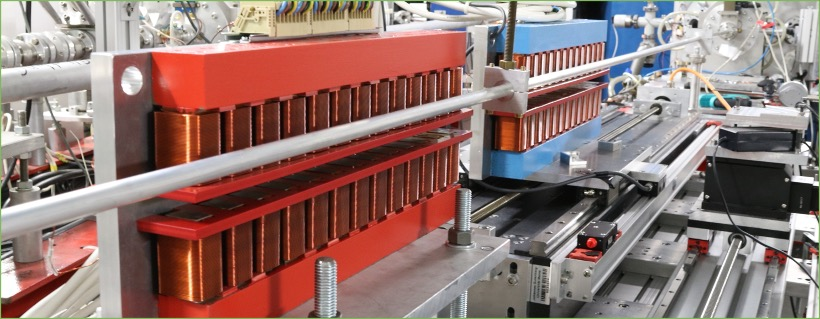
\includegraphics[width=0.8\linewidth]{image/1-1.jpg}\\
  \caption{サンプルの図}
  \label{sample_image}
\end{figure}

\begin{itemize}
  \item a
\end{itemize}
\begin{enumerate}
  \item b
\end{enumerate}

\begin{align}
\frac{1}{2} = \qty(\frac{1}{3}) + \qty{1}\Sigma
\end{align}

\end{document}